\section{System Model}
%----------------------------------------------------------------------------------------%
\subsection{Network Model}
We consider an edge computing system with $K$ Access Points (APs) and $M$ edge servers, which are connected in a network as illustrated in Fig.\ref{fig:system}.
The sets of APs and edge servers are denoted as $\apSet \define \set{1,\dots,K}$ and $\esSet \define \set{1,\dots,M}$, respectively.
Each AP collects the computation jobs from the mobile users within its coverage, and makes decision for each job on which edge server it should be dispatched to.
\accept{In this paper, we shall focus on the decentralized dispatcher design at each AP.}

\begin{figure}[ht]
    \centering
    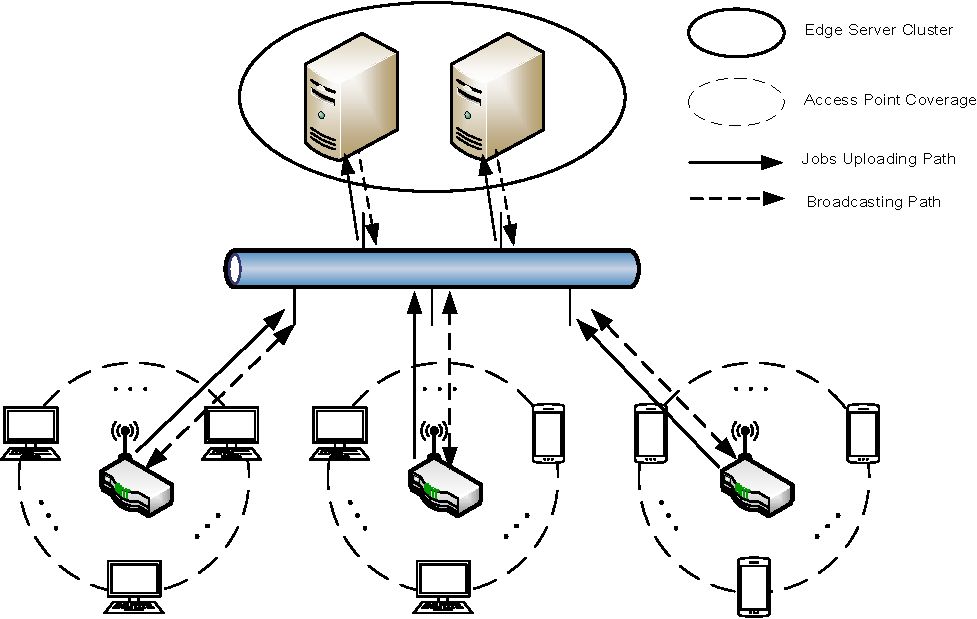
\includegraphics[width=0.80\textwidth]{system-model.pdf}
    \caption{The Illustration of MEC System Model}
    \label{fig:system}
\end{figure}

%NOTE: [job space support and arrival process]
The time axis of each AP is organized by time slots.
Without loss of generality, it is assumed that there are $J$ types of computation jobs supported in this system, which is denoted as $\jSpace \define \set{1,\dots,J}$.
The job arrivals in each time slot are modelled as independent Bernoulli distributions.
More specifically, the arrivals of the $j$-th type of jobs at the $k$-th AP are independent and identically distributed (i.i.d.) Bernoulli random variables, and the arrival probability is denoted as $\lambda_{k,j}$ ($\forall k\in\apSet, j\in\jSpace$).


%NOTE: [uploading process]
Each AP then immediately dispatches each type of received jobs to one edge server.
Let $\omega_{k,j}$ denotes the index of edge server for the processing of the $j$-th types of jobs dispatched from the $k$-th AP ($\forall k\in\apSet, j\in\jSpace$).
Different types of jobs may have different distributions on the input data size.
Moreover, due to the random traffic in the network, the job uploading from one AP to one edge server consumes a random number of time slots.
It's assumed that the distributions of uploading delays are independent between any two uploading jobs.
Hence, we denote $\mathcal{U}_{k,m,j}$ as the uploading delay distribution for the $j$-th type of jobs from the $k$-th AP to the $m$-th edge server, which is ranged in $(0, \Xi]$ with the unit of time slot ($\forall k\in\apSet, m\in\esSet, j\in\jSpace$).
\delete{
    It's assumed that the distributions of uploading delays are independent between any two uploading jobs.
    Denote the uploading delays are i.i.d for the $j$-th type of jobs from the $k$-th AP to the $m$-th edge server, which is denoted as $\mathcal{U}_{k,m,j}$ ranged in $(0,\Xi]$ with the unit of time slot ($\forall k\in\apSet, m\in\esSet, j\in\jSpace$).
}
In practice, the distribution of uploading delay may not be known to the APs or edge servers in advance.

%NOTE: [processing process]
There are $J$ virtual machines (VMs) on one edge server for the computation of $J$ types of jobs.
For each type, the uploaded jobs are computed in a First-Come-First-Serve (FCFS) manner.
Furthermore, we adopt \emph{unrelated machines} assumption in \cite{tan-online} for job processing on edge servers.
The job processing time on different servers are random and machine dependent, which implies that different types of jobs on different edge servers have different processing time distributions.
We denote $\mathcal{C}_{m,j}$ as the processing time distribution of the $j$-th type job on the $m$-th edge serer, whose range is in $(0, c_{m,j}]$ with the unit of time slot ($\forall m\in\esSet, j\in\jSpace$).
The maximum job queue length for each VM is set as $l_Q$, which indicates that there are at most $l_Q$ jobs pending for one VM on the edge servers.
\accept{The jobs submission over the limits would be discarded.}

\delete{We highlight the life cycle of the job being processed.}
%----------------------------------------------------------------------------------------%

\subsection{Periodic Broadcast of State Information}
%NOTE: Periodic Broadcast is Indispensable
In our system, each AP dispatches different types of computation jobs in a cooperative manner, where the jobs are dispatched to achieve a global optimality.
To facilitate such dispatching decision, each AP should collect the information from other APs and edge servers.
It's assumed that every APs and edge servers broadcast their information every $t_B$ time slots as illustrated in Fig.\ref{fig:brd-timeline}.
Furthermore, we denote $t_{i,n}$ as the $n$-th time slot in $i$-th broadcast interval, which is the interval between $(i-1)$-th and $i$-th broadcast ($i=1,2,\dots$).
Especially, we have $t_{i} \define t_{i,0}$ as the index of $i$-th broadcast time slot and call it $i$-th \brpoint~($i=1,2,\dots$).
\begin{figure}[ht]
    \centering
    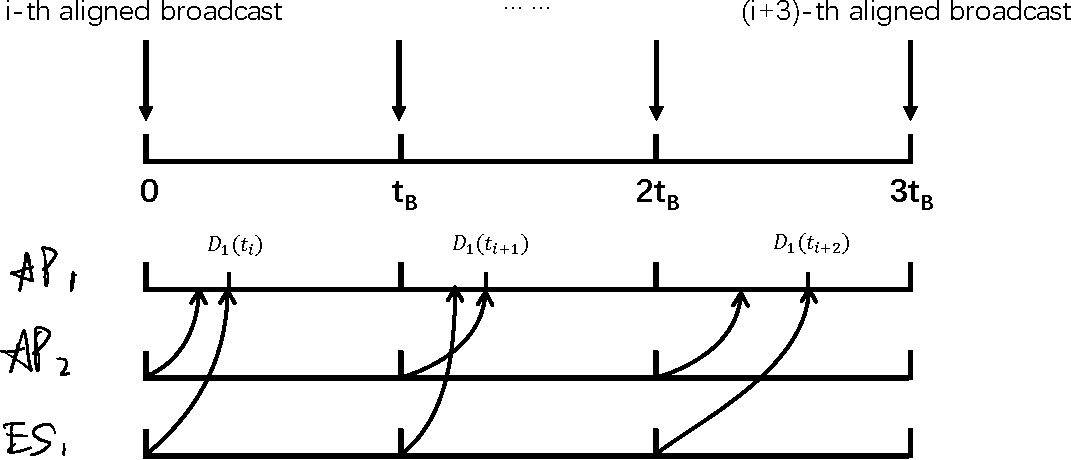
\includegraphics[width=0.80\textwidth]{brd-timeline.pdf}
    \caption{The Timeline Illustration of State Information Broadcast and Receiving}
    \label{fig:brd-timeline}
\end{figure}

%NOTE: State and Broadcast Information for AP
One AP shall maintain information about the number of jobs still in uploading. 
And due to the uploading time of one job is unknown until it's been uploaded, it further has counters to record the elapsed time slots for each job.
More specifically, at $t_{i,n}$ time slot, the number of the $j$-th type job been uploaded to the $m$-th edge server $\xi$ time slots ago from $k$-th AP is denoted as $R^{(k)}_{m,j,\xi}(t_{i,n})$ ($\forall k\in\apSet, m\in\esSet, j\in\jSpace, \xi\in(0,\Xi]$).
The broadcast information of the $k$-th AP at the $i$-th broadcast ($i=0,1,\dots$) is defined as follows.
\begin{align}
    \mathcal{R}_{k}(t_{i}) \define \set{R^{(k)}_{m,j,\xi}(t_{i}) | \forall m\in\esSet, j\in\jSpace, \xi \in [0,\Xi]}.
\end{align}

%NOTE: State and Broadcast Information for ES
One edge server shall maintain information about the queue status for each VM.
More specifically, at $t_{i,n}$ time slot, the $m$-th edge server have $L_{m,j}(t_{i,n})$ and $\eta_{m,j}(t_{i,n})$ denote the pending number and the first job remaining time of the $j$-th type job, respectively ($\forall m\in\esSet, j\in\jSpace$).
The broadcast information of the $m$-th edge server at the $i$-th ($i=0,1,\dots$) broadcast is defined as follows.
\begin{align}
    \mathcal{Q}_{m}(t_{i}) \define \set{Q_{m,j}(t_{i}) | \forall j\in\jSpace},
\end{align}
where $Q_{m,j} \define (L_{m,j}, \eta_{m,j})$.
And the whole broadcast information from all APs and edge servers at the $i$-th broadcast ($i=0,1,\dots$) is denoted as:
\begin{align}
    \Obsv(t_{i}) \define
        \Brace{
            \mathcal{R}_{k}(t_{i}), \mathcal{Q}_{m}(t_{i}) | \forall k\in\apSet, m\in\esSet
        }.
\end{align}

%NOTE: Receiving points definition, denotation and unpredictable
According to Fig.\ref{fig:brd-timeline}, different APs would receive different parts of broadcast information at different time slots.
For $i$-th broadcast ($i=0,1,\dots$), the $k$-th AP would receive the broadcast information from $k'$-th AP after some delay $D^{\dagger}_{k,k'}(t_{i})$, and $D^{\ddagger}_{k,m}(t_{i})$ for the information from the $m$-th edge server ($\forall k' \neq k \in\apSet, m\in\esSet$).
We call the delay after which one AP (saying the $k$-th AP, $\forall k\in\apSet$) could receive the whole broadcast information as \brdelay, which is defined as follows.
\begin{align}
    D_{k}(t_{i}) \define \max\Paren{\Brace{
        D^{\dagger}_{k,k'}(t_{i}),
        D^{\dagger}_{k,m}(t_{i}) | \forall k' \neq k \in \apSet, m\in\esSet
    }}.
\end{align}
Due to the randomness of the network traffic, the \brdelay~shall be random based on the uncertainty of the arrival delay of each partial broadcast information.
Thus APs have i.i.d. distributions of \brdelay, which is denoted as $\mathcal{D}_{k}$ ($\forall k \in \apSet$).
To avoid the \emph{broadcast storm} which could block the normal network traffic, the broadcast should have reasonable period and .
Hence we set the broadcast interval a value always larger than the maximum \brdelay, i.e. $t_B > \hat{D}_k$ ($\forall k\in\apSet$), where $\hat{D}_k$ is the upper bound for $D_{k}(t_{i})$ ($i=1,2,\dots$).

\fixit{
    The broadcast interval selected implies that any AP would receive the whole broadcast information before the next broadcast.
    Due to the complexity of possibilities of partial broadcast information compounds, we consider the time when AP could have a consensus on the whole broadcast information.
    The randomness of \brdelay~implies that one AP could not know other APs' \brdelay~in that interval.
    In the worst case, the APs would always update their dispatching decision only at the end of the interval.
}

In the following problem formulation section, we will show that we could come up with better dispatching decision by awareness of the \brdelay, and improve APs' dispatching decisions in an iterative way.
Furthermore, with the help of algorithm design we could prove that our improved policy is with analytical performance bound under MDP framework.

\delete{
    Due to the introduced periodic broadcasting design and the information receiving delay, this kind of system is inherent of the structure that decisions are always made with obsolete and partial information.
    This implies that: if any AP changes its decision with respect to newly-arrival broadcast information, it will disturb other APs' decisions from cooperation due to different information of system states.
    Thus, it's unacceptable to update APs' policy only when the APs all come up with exactly same information.
}
%----------------------------------------------------------------------------------------%